\documentclass[sigconf]{acmart}
\settopmatter{printacmref=false} % Removes citation information below abstract
\renewcommand\footnotetextcopyrightpermission[1]{} % removes footnote with conference information in first column
\pagestyle{plain} % removes running headers
\makeatletter
\renewcommand\@formatdoi[1]{\ignorespaces}
\makeatother

\usepackage{booktabs} % For formal tables
%\usepackage{indentfirst}
%\usepackage{amsthm}
%\usepackage{amsmath}
%\usepackage{amssymb}
\usepackage{paralist}
%\usepackage{graphicx}
%\usepackage{verbatim}
\usepackage{algorithm}{}
\usepackage{algorithmic}
\usepackage{clrscode3e}
%\newtheorem{mydef}{Definition}
%\newtheorem{theorem}{Theorem}
%\usepackage{amsthm}
\usepackage{subcaption}
\renewcommand{\algorithmicrequire}{ \textbf{Input:}}  
\renewcommand{\algorithmicensure}{ \textbf{Output:}}



% Copyright
%\setcopyright{none}
%\setcopyright{acmcopyright}
%\setcopyright{acmlicensed}
\setcopyright{rightsretained}

%\setcopyright{usgov}
%\setcopyright{usgovmixed}
%\setcopyright{cagov}
%\setcopyright{cagovmixed}


% DOI
\acmDOI{10.475/123_4}

% acmISBN
\acmISBN{123-4567-24-567/08/06}

%Conference
%\acmConference[WOODSTOCK'97]{ACM Woodstock conference}{July 1997}{ElPaso, Texas USA}
%\acmYear{1997}
%\copyrightyear{2016}


\acmArticle{4}
\acmPrice{15.00}

% These commands are optional
%\acmBooktitle{Transactions of the ACM Woodstock conference}
%\editor{Rongkun Yan}
%\editor{Jian Guo}
%\editor{Xiaoran Zhu}
%\editor{Xin Li}
%\editor{Jizheng Ding}


\begin{document}
%\setlength{\baselineskip}{20pt}
\title{Timing Modeling and Analysis for AUTOSAR OS Schedule Tables}
%\titlenote{Produces the permission block, andcopyright information}
%\subtitle{Extended Abstract}
%\subtitlenote{The full version of the author's guide is available as
  %\texttt{acmart.pdf} document}


%\author{Rongkun Yan}
%\affiliation{%
%  \institution{Soft/Hardware Co-design Engineering Research Center, East China Normal University}
%}
%\email{51164500085@stu.ecnu.edu.cn}

%\author{Jian Guo}
%\affiliation{%
%  \institution{Soft/Hardware Co-design Engineering Research Center, East China Normal University}
%}
%\email{jguo@sei.ecnu.edu.cn}

%\author{Xiaoran Zhu}
%\affiliation{%
%  \institution{National Trusted Embedded Software Engineering Technology Research Center, East China Normal University}
%}

%\author{Xin Li}
%\affiliation{%
%  \institution{Shanghai Key Laboratory of Trustworthy Computing, East China Normal University}
%}

%\author{Jizheng Ding}
%\affiliation{%
%  \institution{Soft/Hardware Co-design Engineering Research Center, East China Normal University}
%}



% The default list of authors is too long for headers.
%\renewcommand{\shortauthors}{B. Trovato et al.}


\begin{abstract}
Schedule table mechanism is an important characteristic in AUTOSAR OS during addressing its real-time property and flexibility. Schedule table provides an encapsulation of a statical configuration with one or more actions (i.e., events set or tasks activation). It is challenging to manually analyze schedulability of tasks in schedule tables. In this paper, we take into consideration the AUTOSAR OS scheduling with preemptive periodic schedule tables in uniprocessor. A schedule table is formally modelled by a transition system.
An algorithm based on the models is presented to analyze schedulability by checking all of the possible offsets between schedule tables.
Furthermore, checking schedulability tool is implemented. Testbenches of schedule tables are executed in our tool and an industrial AUTOSAR OS on microcontroller respectively. The result demonstrates our method is effective.
\end{abstract}

%
% The code below should be generated by the tool at
% http://dl.acm.org/ccs.cfm
% Please copy and paste the code instead of the example below.
%


%\ccsdesc[500]{Computer systems organization~Embedded systems}\ccsdesc[300]{Computer systems organization~Redundancy}\ccsdesc{Computer systems organization~Robotics}\ccsdesc[100]{Networks~Network reliability}


%\keywords{ACM proceedings, \LaTeX, text tagging}


\maketitle

\section{Introduction}
Formal methods have been widely and successfully applied to functional properties verification. But unfortunately, it is difficult to verify some non-functional characteristics, which are the key to maintain validity in highly safety-critical real-time systems. Formal analysis on schedulability of task models is researched. Liu et. al \cite{DBLP:journals/jacm/LiuL73} first build a task model for periodic tasks with a period and execution time and discuss two scheduling algorithms over the model. Stigge et al. \cite{DBLP:conf/rtas/StiggeEGY11} describe a task with a Diagraph Real-Time (DRT) task model and study the feasibility problem on preemptive periodic tasks in a uniprocessor. For analyzing the temporal validity of real-time data objects, Wang et al. \cite{DBLP:journals/computing/WangLHSM13} give transaction model with three parameters, a fixed priority, worst-case execution time (WCET) and a relative deadline. The temporal validity of real-time data object is  analyzed by periodic update transactions. S.Baruah \cite{DBLP:conf/rtss/Baruah16} analyze schedulability in a general 3-parameter sporadic task model \cite{DBLP:journals/csur/BurnsD17} for mixed-criticality concurrent real-time tasks. Moreover, S.Baruah et al. \cite{DBLP:conf/rtns/2017} propose a scheduling model for periodic preemptive tasks inspired by control theory. Despite the rapid advancements in real-time scheduling theory, industry is willing to employ the very simple cyclic executive approach \cite{DBLP:journals/rts/BakerS89} for corrective scheduling to meet stringent certification requirement. C.Deutschbein et al. \cite{DBLP:conf/setta/2017} present the problem of constructing cyclic executive upon multiprocessors.

AUTOSAR (AUTomotive Open System ARchitecture) \cite{autosar} is an open and standardized layered software architecture and interfaces. The integration of software modules from different vendors forms the complete architecture. %As a consequence, more and more automotive companies tend to take AUTOSAR as their primary standard for developing their base software project, such as operating system. 
Researchers working on AUTOSAR OS are rich in progressive and proactive. There have been many studies on analyzing AUTOSAR OS specification \cite{DBLP:conf/isorc/AnssiTKGT11}. 
%Peng et al. adopt timed CSP method to model OS and the engine management system (EMS), some safety properties based on CSP models are verified through process analysis toolkit in \cite{DBLP:conf/tase/PengHSG13}. Huang et al. \cite{DBLP:conf/icfem/HuangFHQH13} apply formal semantics to describing tasks in AUTOSAR OS with time protection mechanism. The model predicts whether a task would violate its time constraint, and is implemented in Mathematica tool with a case study. Zhu et al. \cite{DBLP:conf/tase/ZhuLSWZ13} focus on the timing properties of AUTOSAR OS and propose an automatic verification framework based on rewriting logic to analyze the timing behaviors. Therefore, many researches of AUTOSAR OS focus on its specification, implementation and verification. 
For schedulability of the AUTOSAR OS, both Zhao et al. \cite{DBLP:journals/jsa/ZhaoGZ17} and Hatvani et al. \cite{DBLP:conf/etfa/HatvaniB15} adopt preemptive threshold to improve the schedulability. Tasks are set with a higher priority and reduced execution time by the stack usage. In order to assist developers to assign the priorities of tasks, Yoon et al. \cite{DBLP:conf/racs/YoonR14} present a real-time task chain model, which helps to obtain a near-optimal priority assignment from the model. They concentrate on the scheduling of tasks, but few researches deal with schedule tables. Wang et al. propose a method for generating schedule tables containing periodic tasks with dependence in \cite{DBLP:conf/dasip/WangCM16} for the multi-core architectures. However the method does not give the correctness proof of generating schedule tables.

Among those aforementioned researchers, most of them analyze schedulability by modeling tasks, few attentions were given to schedule table mechanism \cite{autosar}, which is an important mechanism in AUTOSAR OS. For automobile being a high safety-critical real time system, a practical approach \cite{DBLP:journals/rts/BakerS89} applies to schedule tables in order to satisfy all tasks deadline. Inspired by the method, we present a formal method to build deterministic schedule tables. The correctness of these deterministic schedule tables is proved, which means to verify every task in schedule tables meets its deadline.

A formal model is constructed for each schedule table. A set of schedule tables are composed by concurrent of all models. Tasks in schedule tables are static analyzed to prove that whether tasks finish in deadline. We propose an algorithm to travel all of the possible schedule situations so that each situation can exactly complete task execution. A time interval between a task releasing and its deadline is checked to confirm whether enough execution time for itself and other higher priority tasks. Because all schedule tables in this method are periodic, analysis of infinite running of tasks is transformed to finite running of tasks by introducing hyperperiod of schedule tables. In addition, after analyzing the schedulability of a set of schedule tables by our approach, we run testbenches of schedule tables on an implemented AUTOSAR OS based on TC1782 32-Bit Single-Chip Micro-controller \cite{infineon.org}. The result shows the consistency between them.


The rest of this paper is organized as follows. Section 2 introduces some concepts of AUTOSAR and schedulability analysis. Section 3 discusses the constraints of AUTOSAR OS in this paper and describes our formal models of schedule tables. Section 4 presents some definitions and notations of our algorithm. In Section 5, we propose a method by integrating concepts in section 4. Then, we compare the result of our method with the execution on hardware in Section 6. Finally, in Section 7, we give the conclusion and future work.
\section{Background}
For a better understanding of our work, we give a brief overview of AUTOSAR operating system and methods of schedulability analysis.
\subsection{AUTOSAR Operate System}

AUTOSAR considers a task as the minimum unit to schedule. Even a simple application also needs to map to a task. Each task has to accomplish a specific function. The implementation of a task consists of a block of sequential code. AUTOSAR provides two types of tasks: extended and basic tasks.

Each basic task has three states: $running$, $suspended$ and $ready$. A task in the $running$ state is executed by processor. A suspended task can be put into ready queue by a system service which will transfer the task into $ready$ state. A task in $ready$ state is waiting for allocation of the processor. At most one task can be in $running$ state at the same time. Once a basic task in $running$ state is preempted by a task with a higher priority, it will be transferred into $ready$ state. A running task is transferred into $suspended$ state by a system service to terminate a task. An extended task has a strong resemblance to a basic task with except that 1) the former one could wait for a system event in an extra state named $waiting$, 2) the basic task is allowed to be activated once or multiple times while an extended task can only be activated once. 

AUTOSAR uses the highest priority first and first come first served as its scheduling policy. AUTOSAR reserves a FIFO queue for each priority. When a task is activated, it will be put into the corresponding queue. Then scheduler will detect those queues in order of the highest priority and choose the task with the highest priority to execute. If more than one tasks in ready queue have the highest priority, the scheduler will choose the first one has been put into the ready queue. For the high efficiency of the system, the priorities are distributed to tasks statically.

The schedule table mechanism is a new concept introduced in AUTOSAR which could statically define the pattern of tasks activation. Each schedule table encapsulates a predefined set of expiry points. An expiry point contains one or more actions which can be either activating a task or setting an event. Each expiry point has a unique offset in ticks from the start of the schedule table. In addition, a schedule table has a specific duration which defines the modulus of the schedule table. The process of schedule tables can be manipulated as users call system services at any time.

AUTOSAR offers two types of behavior of schedule tables: single-shot and repeating. On one hand, if a schedule table is configured as single-shot, it will stop after the final expiry point is processed. On the other hand, for a repeating schedule table, after the final expiry point has been processed, it loops back to the first expiry point. Note that for tasks activated by a repeating schedule table, they can be regarded as periodic tasks and their period equals to the duration of the repeating schedule table. We give an example in Figure \ref{figure_st1} to illustrate the construction of schedule table. This schedule table is denoted by $st_1$ with the duration of 17 ticks.
\begin{figure}[t]
  \centering
  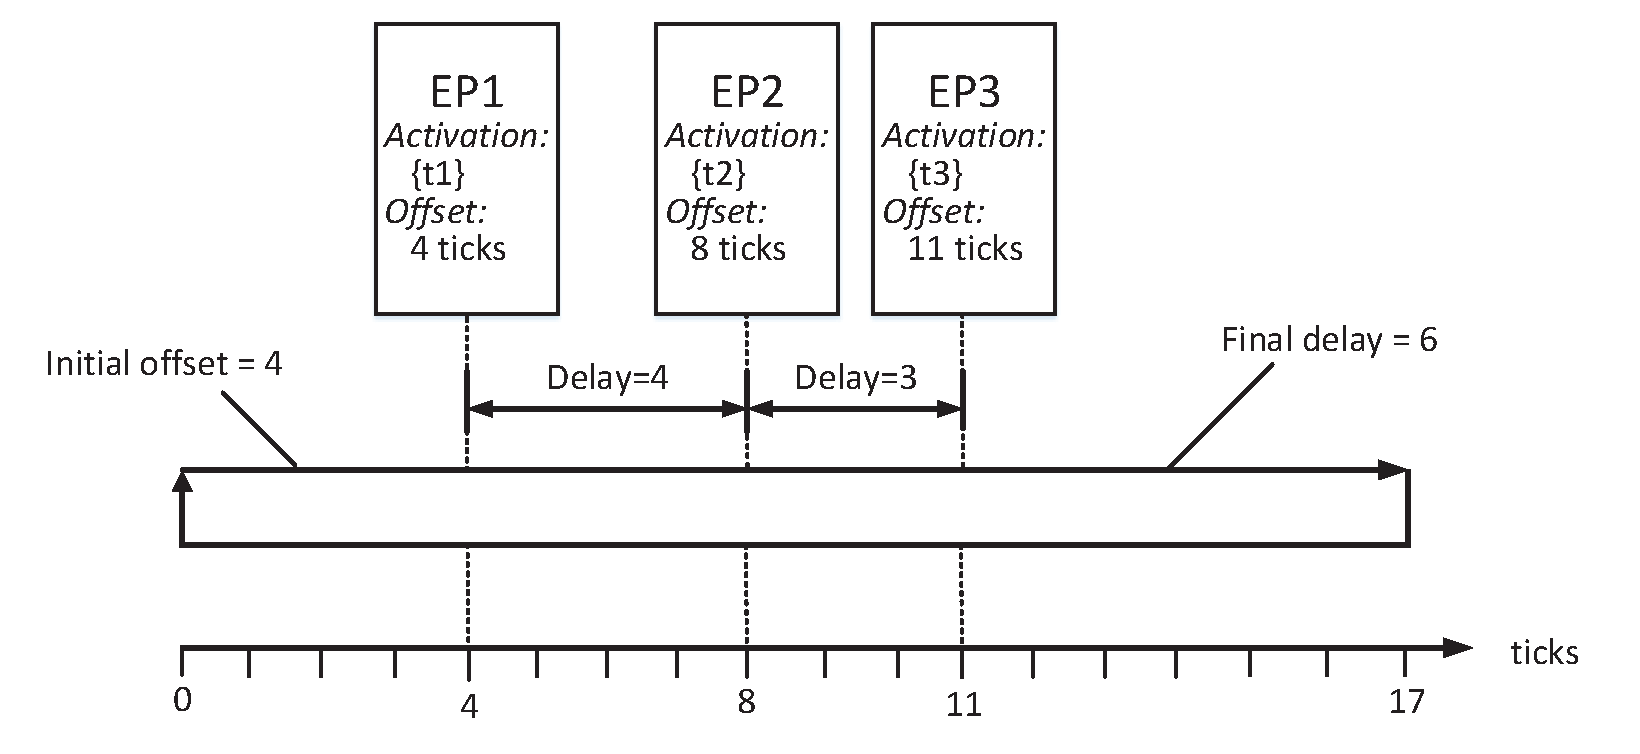
\includegraphics[scale=.32]{graphics/figure_st1.eps}
  \caption{An example repeating scheduel table cotaining three expiry points, and $t_1,t_2,t_3$ is three tasks.}
  \label{figure_st1}
\end{figure}

\subsection{Schedulability Analysis}
The researches about schedulability analysis focus on the problem whether real-time tasks could satisfy its time property. We declare the meaning of schedulability: schedulability declare whether a set of schedule tables is schedulable. Schedulable means all tasks activated by schedule tables could take to execute before its deadline, otherwise, this set of schedule tables is non-schedulable.

In order to figure out the schedulability of real-time systems, several theories have been presented. We can categorize those methods by the existing scheduling algorithm. One of the most common algorithm is the earliest deadline first algorithm (EDF). EDF is considered as an optimized algorithm on preemptive uniprocessors to analyze a set of independent tasks characterized by activate time, deadline and worst case execution time. For such a dynamic priority scheduling algorithm, the schedulability analysis methods which determines whether a system is EDF schedulable is co-NP in the strong sense \cite{Goossens:1999:LWC:553897}.

Since our work focuses on the single processor platform with static priority scheduling, we now pay attention the schedulability analysis method based on the response time analysis (RTA) \cite{DBLP:journals/iee/AudsleyBRTW93}. Response time analysis is suited for fixed priority tasks system. This method calculate the worst case response time, then verify whether the worst case response time of a task is in its deadline. 

\section{Formal models of schedule tables} 
For AUTOSAR operating system, there are two main factors that make the schedulability analysis intractable: 1) in AUTOSAR, several schedule tables run concurrently, 2) users can manipulate the proceeding of schedule tables by calling system services, i.e., schedule tables may stop or start running at any time, which is totally unpredictable. In order to resolve this, we decide to define a proper formal model to describe the behavior of schedule tables, then propose an algorithm to analyse the schedulability of schedule tables by the formal model. In this section, we state our model firstly. 

\subsection{Constraints of AUTOSAR OS}
On account of the widespread use of embedded automotive systems, different embedded applications may require various characteristics of operating systems as well as hardware environments are also likely to be different. So AUTOSAR provide various features to satisfy requirements. Among them, our work only focus on several characteristics: 
\begin{compactenum}
  \item Tasks are allowed to share the same priority level
  \item Lower number for higher priority.
  \item We take no account of extended tasks and events.
  \item All tasks are full preemptible.
  \item The first scheduling policy is highest priority first, the second policy is first come first served.
  \item A basic task can be activated infinitely many times. 
\end{compactenum}

For convenience, if a task is assigned to more than one expiry points, we regard them as different tasks. In additional, we assume all schedule tables are repeating. In fact, a repeating schedule table could be transferred to a single-shot schedule table by converting the final delay into infinitely great.

\subsection{Formal Models}
We use a directed digraph to describe the behavior of a schedule table and named it Digraph Schedule Table model (DST). Each DST is a tuple $(Node,Tasks,Act,\rightarrow,Delay)$, where
\begin{compactitem}
  \item $Node$ is a finite set of expiry points.
  \item $Tasks$ is a finite set of tasks. We use a tuple $(e,d,l)$ to represent a task. Assuming $t_k\in Tasks$, then $e(t_k),d(t_k),l(t_k)$ denote the execution time, deadline and priority level of task $t_k$ respectively.% In the beginning, release time of all tasks set to 0, and could be modified during verify procedure.
  \item $Act$ : $Node \rightarrow 2^{Tasks}$ is a function. $Act$ relates a set of actions $Act(ep)\in 2^{Tasks}$ to an expiry point $ep$.
  \item $\rightarrow\ \subseteq Node\times Node$ is a transition relation to describe the execution sequence of expiry points. 
  \item $Delay$ : $Node \rightarrow ticks$ is a function to describe the delay after processing an expiry point. $Delay$ of the last expiry point equals to the final delay plus the initial offset.
\end{compactitem}

Note that we conceal the initial offset in DST. Because during the running of a repeating schedule table, except the first loop, the initial offset always can be considered as a part of the delay of the last expiry point. With regard to the definition of $Delay$, the duration of a schedule table can be obtained by 
\[\delta(DST)=\sum\limits_{ep_i\in Node}Delay(ep_i).\]

During the execution of a schedule table, expiry points will expire circularly. We record each time of expiring as an instance of expiry point. An instance of expiry point is represented by a pair $(ep_i,r_i)$, where $r_i$ is the expiry time. 
Naturally to point out that the execution of a DST corresponds to an infinite sequence of instances of expiry points. 
We use a path $\rho=[(ep_1,r_1),(ep_2,r_2),\dots,(ep_k,r_k)]$ to describe a fragment of an execution. When an expiry point expire, corresponding tasks will be activated then. For each time a task is activated, we record that as an instance of task. We use a 4-tuple $(e_i,d_i,l_i,r_i)$ to denote an instance of a task with execute time $e_i$, deadline $d_i$, priority $l_i$ and activate time $r_i$. Durning a path, expire times of instances of expiry points are constrained by the delay of corresponding expiry points, i.e., 
\[r_{i+1}=r_i+Delay(ep_i).\]

Similar to the calculation of duration, we get the length of a path by accumulating delays of expiry points. For a path $\rho=[(ep_1,r_1),(ep_2,r_2),\dots,(ep_k,r_k)]$, the length is calculated by: \[\iota(\rho)=r_k-r_1.\]


\subsection{Example Model}\label{section_dst_1}
We model the schedule table given before as Figure \ref{figure_dst1} and give the tuple as follow.
\begin{figure}
  \centering
  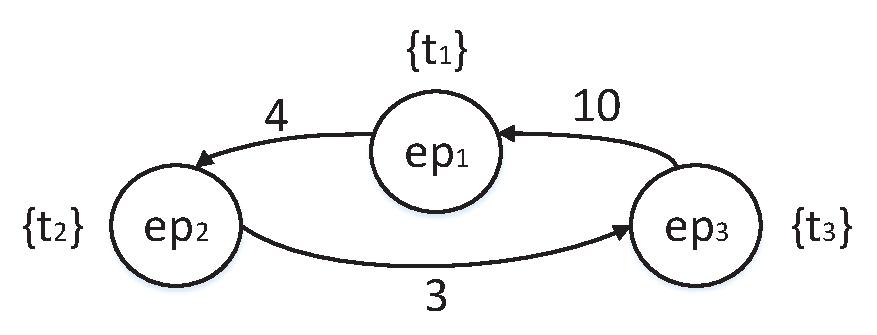
\includegraphics[scale=.4]{graphics/figure_dst1.eps}
  \caption{An example of DST for $st_1$, where $t_1=<2,4,2>,\ t_2=<2,3,1>\ t_3=<2,9,6>$.}
  \label{figure_dst1}
\end{figure}

$dst_1=\{Node_1,Tasks_1,Act_1,\rightarrow_1,Delay_1\}$, where 
\begin{compactitem}
\item $Node_1=\{ep_1,\ ep_2,\ ep_3\}$ which cotains all expiry points.
\item $Tasks_1=\{t_1,\ t_2,\ t_3\}$ which cotains all tasks in $dst_1$.
\item $Act_1$ refers to actions of an expiry point:$Act_1(ep_1)=t_1$, $Act_1(ep_2)=t_2$, $Act_1(ep_3)=t_3$.
\item $\rightarrow_1=\{(ep_1,ep_2),(ep_2,ep_3),(ep_3,ep_1)\}$ which shows the execution sequence of expiry points.
\item $Delay_1:$ the $Delay$ of expiry points is defined by $Delay_1(ep_1)=4$, $Delay_1(ep_2)=3$, $Delay_1(ep_3)=10$.
\end{compactitem}

%The duration of $dst_1$ \[\delta(\rho)=Delay(ep_1)+Delay(ep_2)+Delay(ep_3)=17.\]
%We assume there is a path $\rho$ over $dst_1$ which $\rho_1=ep_1$ and $r_1=0$. The expire time of second instance of expiry point is $0+Delay(ep_1)=4$. If $\rho=[(ep_1,0),(ep_2,4),(ep_3,7),(ep_1,17)]$, the length of $\rho$ can be calculated by\[\iota(\rho)=Delay(ep_1)+Delay(ep_2)+Delay(ep_3)=17.\]

\section{Definition and notation}\label{section_definition}
In this section, we discuss how to verify whether a task could always satisfy its time property. We start this by introducing some concepts as preparations, then integrate those concepts into a complete method.

\subsection{Computational Requirement}
The main idea of our analysis method is to check whether the time interval between a task's activation and deadline is big enough to accommodate the execution time of itself and other tasks which could interrupt it. But how to delineate the execution time of tasks could interrupt?

For example, if we are testing an instance of task $(e(t),d(t),l(t),r(t))$, in consideration of the features of schedule policy, this instance could not be interrupted by tasks with a lower priority than $l(t)$, or tasks which have priority $l(t)$ but activate time is larger. Based on this, we introduce the concept of computational requirement to accumulate the execution time on an expiry point and dismiss the tasks which could not affect this instance.
\begin{definition}
For an instance of expiry point $(ep,r)$, we use computational requirement $\omega_{l(t),r(t)}^{(ep,r)}$ to accumulate the execution time of tasks in $Act(ep)$. If $r\leq r(t)$, we remove those tasks which have a lower priority than $l(t)$ from $\omega_{l(t),r(t)}^{(ep,r)}$; when $r>r(t)$, we remove tasks which have priority lower than or equal to $l(t)$ from $\omega_{l(t),r(t)}^{(ep,r)}$:
\begin{equation}
\omega_{l(t),r(t)}^{(ep,r)}=\sum\limits_{task\in \xi_{l(t),r(t)}(ep)}e(task),
\end{equation}\label{equation_loweromega}
where 
\[
\xi_{l(t),r(t)}((ep,r))=\begin{cases}\{t'|t'\in Act(ep)\wedge l(t')\leq l(t)\}\qquad if\ r\leq r(t)\\
\{t'|t'\in Act(ep)\wedge l(t')<l(t)\}\qquad if\ r>r(t)
\end{cases}\]
\end{definition}
After proposing the computational requirement function, the execution time during a path can be computed as well. We still use the name $computational\ requirement$ to denote this function, but a different way to calculate.
\begin{definition}
For a path $\rho=[(ep_1,r_1),(ep_2,r_2),\dots,(ep_n,r_n)]$, we use computational requirement $\Omega_{l,r}(\rho)$ to calculate how long those expiry points on this path will take to execute and only consider the tasks which could affect an instance of task $(e,d,l,r)$:
\begin{equation}
\Omega_{l,r}(\rho)=\sum_{i=1}^n\omega_{l,r}^{\rho_i},
\end{equation}\label{equation_higheromega}
where we use $\rho_i$ to represent the $i$th instance of expiry point on the path $\rho$.
\end{definition}

\subsection{Request Function}\label{section_prf}
Due to the speciality of schedule table mechanism, after an expiry point expires, other expiry points cannot expire during delay time. We extend the prefix request function $prf^{ep}_{l,r}(\theta)$ from \cite{DBLP:journals/rts/Stigge015a}  to abstract the relation between length and computational requirement of paths.
\begin{definition}
For an expiry point $ep$, let prefix request function $prf^{ep}_{l,r}(\theta)$ denotes the maximal computational requirement $\Omega_{l,r}(\rho)$ among those paths $\rho$ which start by $(ep,0)$ and $\iota(\rho)<\theta$.
\begin{equation}
prf^{ep}_{l,r}(\theta)=max\{\Omega_{l,r}(\rho)|\rho \ start\ in\ (ep,0)\ \wedge\ length(\rho)<\theta\}.
\end{equation}\label{equation_prf}
\end{definition}

Beacuse no path has a length which is less than 0, we consider the prefix request function is meaningless when $\theta=0$.

%Regarding expiry point $ep$ in Figure \ref{illustration} as the superscript of prefix request function, we will get the result as the computational requirement of part B, the part C could be seek in a similar way. In a time interval, $ep$ is the start expiry point, $l$ is a priority level, and $r$ is release time. Only tasks with higher priority or not later release time, their execution time could be consider. Independent variable $\theta$ represent the length of time interval.

\begin{figure}[t]
  \centering
  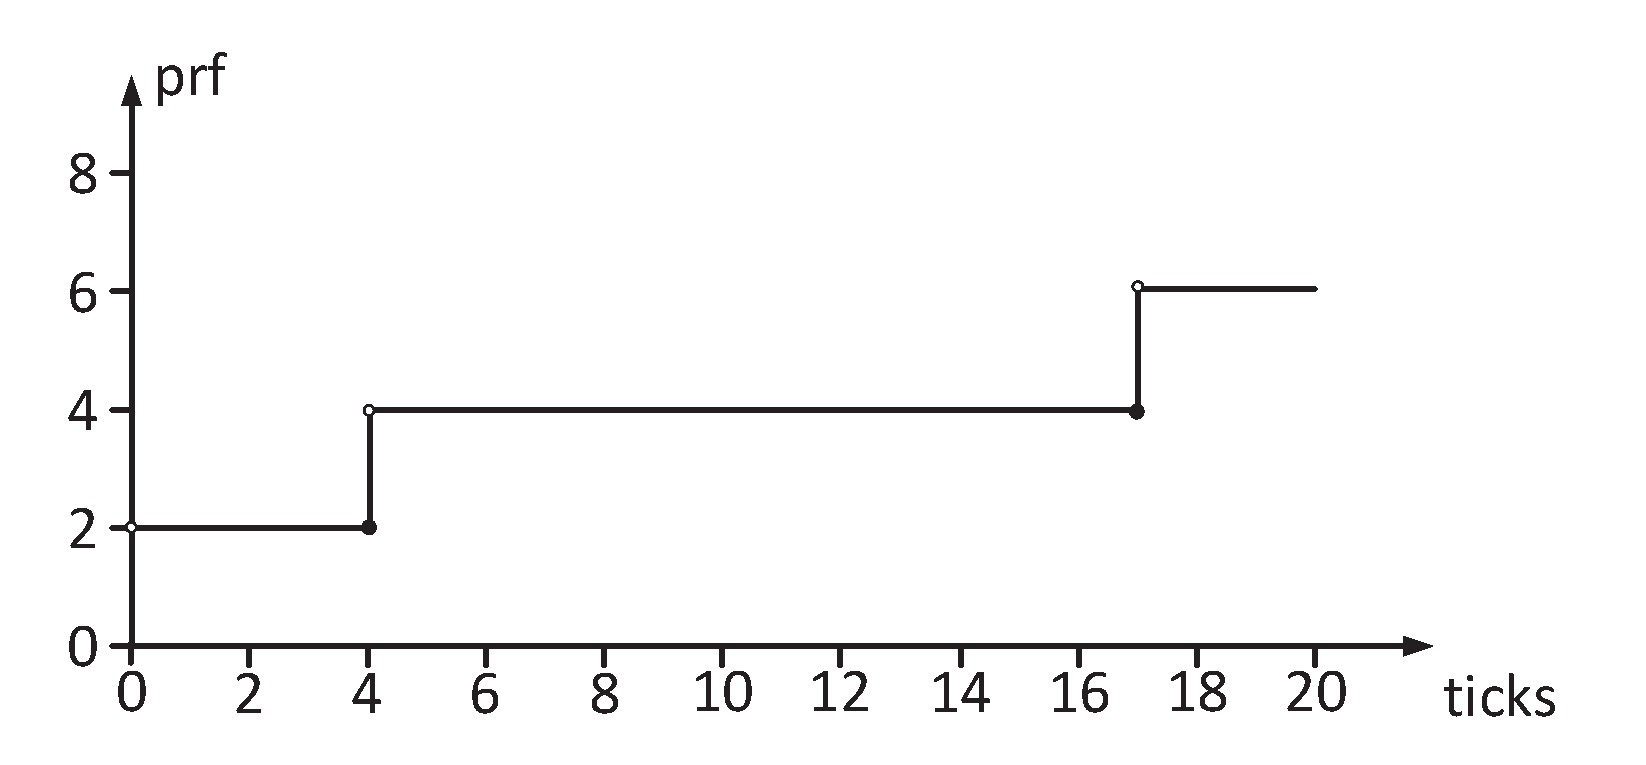
\includegraphics[scale=0.32]{graphics/figure_prf.eps}
  \caption{An example for prefix request function of $prf^{ep_1}_{4,0}(\theta)$ according to $dst_1$ in Figure \ref{figure_dst1}.} 
  \label{figure_prf}
\end{figure}

Figure \ref{figure_prf} shows an example of prefix request function $prf^{ep_1}_{4,0}(\theta)$ (cf. Section \ref{section_dst_1}). When $0<\theta\leq4$, the path must be $[(ep_1,0)]$, which have computational requirement as 2. When $4<\theta\leq7$, the path $[(ep_1,0),(ep_2,4)]$ makes the maximum computational requirement 4. When $7<\theta\leq17$, the path $\rho$ also can be $[(ep_1,0),(ep_2,4),(ep_3,7)]$. But in $ep_3$, the priority of $t_3$ is lower than 4, so the prefix request function wouldn't accumulate it. The function will keep returning 4 until $\theta$ exceeds 17.

A DST has as many prefix request functions as expiry points in this DST, those prefix request functions can be synthesized as one. We use the maximal request function to integrate those prefix request functions.
\begin{figure}
  \centering
  \begin{subfigure}[t]{3.25in}
    \centering
    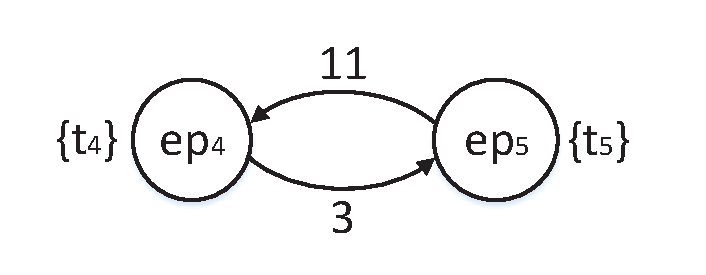
\includegraphics[scale=.45]{graphics/figure_dst2.eps}
    \caption{An example of $dst_2$ which contains two expiry points and $t_4=<1,3,3>,\ t_5=<3,8,5>$.}\label{figure_dst2}
  \end{subfigure}
  \quad
  \begin{subfigure}[t]{3.25in}
    \centering
    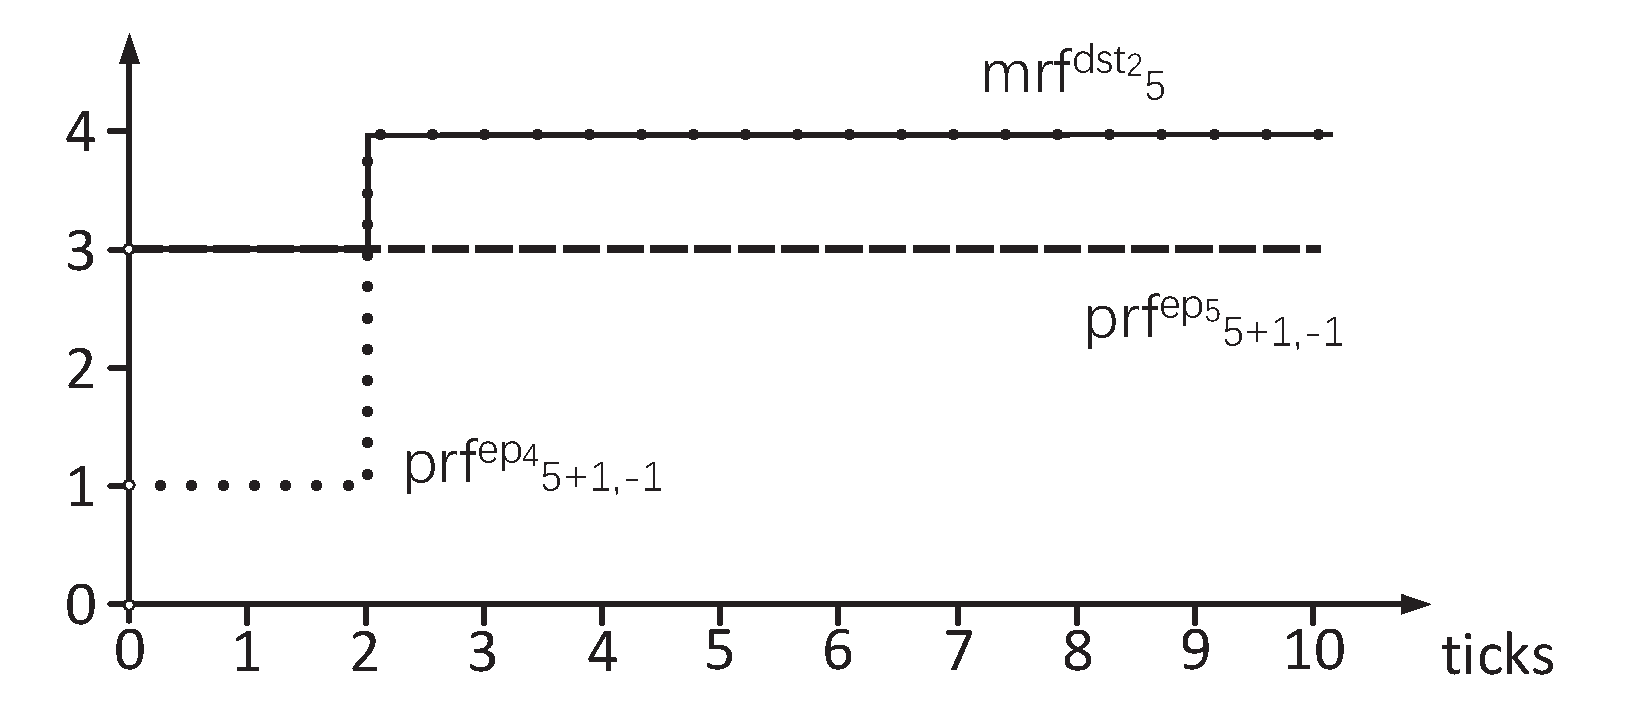
\includegraphics[scale=.325]{graphics/figure_mrf.eps}
    \caption{Maximal request funciton of $dst_2$ for $l=5$.}\label{figure_mrf}
  \end{subfigure}
  \caption{The $dst_2$ contains two expiry points, so there are two prefix request functions $prf^{ep_4}_{5+1,-1}$ and $prf^{ep_5}_{5+1,-1}$ in Figure \ref{figure_mrf}. When $0<\theta\leq2$, $prf^{ep_5}_{5+1,-1}$ makes more computational requirement. But in time interval (2,10], $prf^{ep_4}_{5+1,-1}$ provides the value of the maximal request function.}\label{figure_dst2_mrf}
\end{figure}
\begin{definition}
For a DST, the maximal request function $mrf^{dst}_l(\theta)$ calculates the maximum execution time caused by a time interval with length $\theta$.% prefix request function among expiry points in a DST.
\begin{equation}
mrf^{dst}_l(\theta)=max\{prf^{ep}_{l+1,-1}(\theta)|ep\in Node\}
\end{equation}\label{equation_mrf}
\end{definition}

An example of a maximal request function is given in Figure \ref{figure_dst2_mrf}, where we provide another DST $dst2$ and illustrate the maximal request function of $dst_2$. Notice that in any point of $\theta$, there are at least one prefix request function offer the value of the maximal request function.

Besides considering paths which start with a specific expiry point, we also calculate the computational requirement of paths which end up in a specific expiry point $ep$ which is calculated by the suffix request function \cite{DBLP:journals/rts/Stigge015a}. A slightly different between $srf$ and $prf$ is that the former ignores the expire time.% because all tasks considered in the suffix request function are activated earlier than tasks in $ep$.

\begin{definition}
For an expiry point $ep$, we use a suffix request function $srf^{ep}_{l}(\theta)$ to calaulate the maximal computational requirement $\Omega_{l+1,-1}(\rho)$ among those paths ending up in $(ep,r)$ but whose length not exceeds $\theta$.
\begin{equation}
srf^{ep}_l(\theta)=max\{\Omega_{l+1,-1}(\rho)|\rho\ end\ in\ (ep,r)\ \wedge\ length(\rho)\leq \theta\}.
\end{equation}\label{equation_srf}
\end{definition}
\begin{figure}[t]
  \centering
  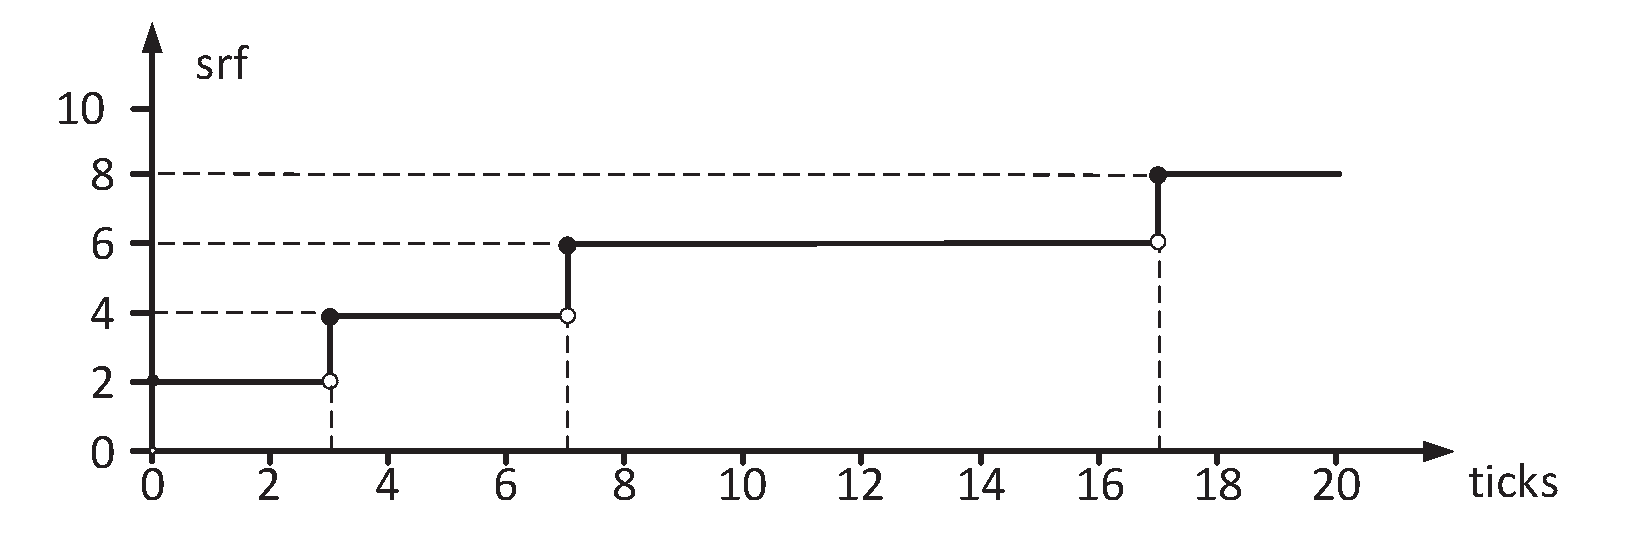
\includegraphics[scale=0.31]{graphics/figure_srf.eps}
  \caption{Suffix request function of $srf^{ep_3}_{4}(\theta)$ according to $DST_1$ in Figure \ref{figure_dst1}.} 
  \label{figure_srf}
\end{figure}

In particular, we use $\Omega_{l+1,-1}(\rho)$ to accumulate the execution time of tasks which have priority not lower than $l$, regardless the activate time. We use Figure \ref{figure_srf} to illustrate the suffix request function $srf^{ep_3}_{4}(\theta)$. Figure \ref{figure_srf} illustrates $srf^{ep_3}_{4}(\theta)$. When $\theta$ start from 0, we calculate the computational requirement of path $[(ep_3,r_3)]$ and get $2$ as the result. When $\theta$ reaches 3, path $[(ep_3,r_3)]$ and $[(ep_2,r_2),(ep_3,r_3)]$ meet the requirement and we choose the maximum value of computational requirement as 4. The rest may be deduced by analogy.

%Suffix request function describes the execution time of all tasks may block task $t$ in schedule table $st$ directly or indirectly, i.e., tasks which release earlier than task $t$, and have higher priority. before and not later than the task need to be verified.Note that the relationship between result of prefix request function and corresponding time $t$ reveal the computational requirement in time interval which length is $t$. 

\subsection{Busy Window}\label{section_busywindow}

A RTOS (Real-Time Operating System) strictly requires that the finish times of tasks are not allowed to exceed deadline. But in real life, identifying the task which causing time fault actually may be far from obvious. Imagine a task which takes too long to execute, but it does not violate its deadline. The task may block the execution of following tasks. Then the influence will spread throughout the running of tasks, which could makes a normal task misses its deadline. But in a execution of a DST, how to recognize those tasks which could cause or spread influences? 
In order to find a solution to this problem, we introduce the well-known concept named busy window \cite{DBLP:conf/rtss/Lehoczky90}. 

Busy window for priority level $l$ is a time interval where processor continuously executes tasks with priority $l$ or a higher priority. If we find the maximal busy window for $l$, then we could delimit how long a task could spread influence, i.e., an instance of task with priority $l$ can only be affected by tasks within this boundary. We denote the upper bound of busy window for $l$ by $\sigma_l$.

\begin{lemma}
For a DST set $\tau$, we can get the upper bound of busy windows for $l$ by finding the minimum positive number $\theta$ which could satisfy
\begin{equation}
\sum\limits_{dst\in \tau}mrf^{dst}_l(\theta)=\theta.\label{equation_busywindow}
\end{equation}
\end{lemma}\label{lemma_busywindow}
\begin{proof}
Firstly, we state a fact that at least one expiry point expire at the point of a busy window start. So the computation of the upper bound of busy windows is all about finding those expiry points which is named as start expiry points.

If there is a $\theta$ satisfies Equation \ref{equation_busywindow}, then for each maximal request function, at least one prefix request function offer its value at $\theta$. We pick any one prefix request function from a maximal request function, then a set of expiry points is obtained as superscript of those prefix request functions. When those expiry points expire at the same time, we can get the upper bound of busy windows for $l$.

Now assuming we use this method and get an expiry point $ep'$ in $dst'$ as start expiry point. But there is another expiry point $ep''$ in $dst'$ which could make a longer busy window. Because the prefix request function of $ep''$ does not offer the value of $mrf^{dst'}_l$ at $\theta$, i.e.,
\[prf^{ep''}_{l+1,-1}(\theta)<prf^{ep'}_{l+1,-1}(\theta).\]
When we choose $ep''$ instead of $ep'$ to expire with other expiry points simultaneously, the sum of the prefix request function is less than $\theta$, i.e., 

\begin{equation}
prf^{ep''}_{l+1,-1}(\theta)+E<prf^{ep'}_{l+1,-1}(\theta)+E=\theta, 
\end{equation}
where $E=\sum\limits_{dst\in \tau-d1}mrf^{dst}_l(\theta)$.

So when $ep''$ expires with other expiry points, the busy window is shorter than $\theta$, leading to a contradiction.
\end{proof}

In some non-schedulable cases, the upper bound of busy windows is infinitely great. In order to recognize this situations, we introduce the definition of the hyperperiod of DSTs as follow.
\begin{definition}
For a set of DSTs $\tau=\{dst_1,dst_2,\dots,dst_n\}$, we assume durations of them as $\delta_1,\delta_2,\dots,\delta_n$ respectively. The hyperperiod is the least common multiple of all duration of all schedule tables as $lcm(\delta_1,\delta_2,\dots,\delta_n)$.
\end{definition}

\begin{lemma}
  A finite set of schedule tables is non-schedulable if there is a busy window exceeds hyperperiod of those schedule tables.
\end{lemma}\label{lemma_hyperperiod}
\begin{proof}
  The scheduling process of a set of repeating schedule tables is cyclic. If any busy window exceeds the hyperperiod, the processor cannot finish those tasks which are activated in this hyperperiod. In the next hyperperiod, except tasks which is activated in this hyperperiod, the processor also has to execute those tasks unfinished. So the tasks with the lowest priority must be blocked. By parity of reasoning, the task with the lowest priority must violate its deadline at some point.
\end{proof}
\subsection{Combination of Expiry Points}\label{section_combination}
In order to achieve completeness in schedulability analysis, our method needs to completely cover every schedule situations, including all offsets between schedule tables. Assuming there is a set of DST $\tau=\{dst_1,dst_2,\dots,dst_n\}$, the amount of offsets between those schedule tables equals to $\delta(dst_1)\times\delta(dst_2)\times\dots\times\delta(dst_n)$. The various offsets may lead to state explosion, so we try to mitigation this problem by using expiry points to represent offsets.

Because our schedulability analysis method always focuses on the execution time, so we measure a time interval with computational requirement. If computational requirement which is caused during a time interval is lager than or equal to other intervals, we say this time interval dominates the others, cf. Figure \ref{figure_combination}.


\begin{figure}  
  \centering
  \begin{subfigure}[t]{3.33in}
    \centering
    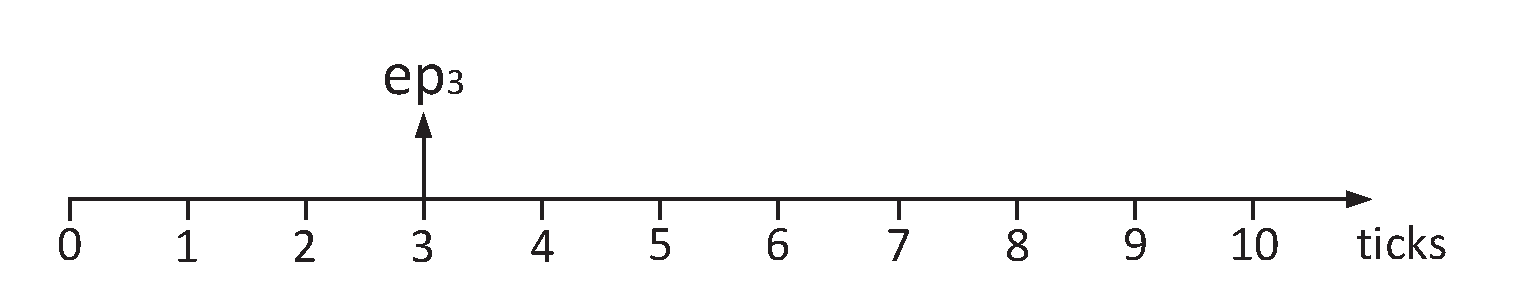
\includegraphics[scale=.34]{graphics/figure_combina2.eps}
    \caption{$ep_3$ expires at 3, the computational requirement which is caused during this time interval is $\omega_{l,r}^{(ep_3,3)}.$}\label{figure_combination1}
  \end{subfigure}
  \quad
  \begin{subfigure}[t]{3.33in}
    \centering
    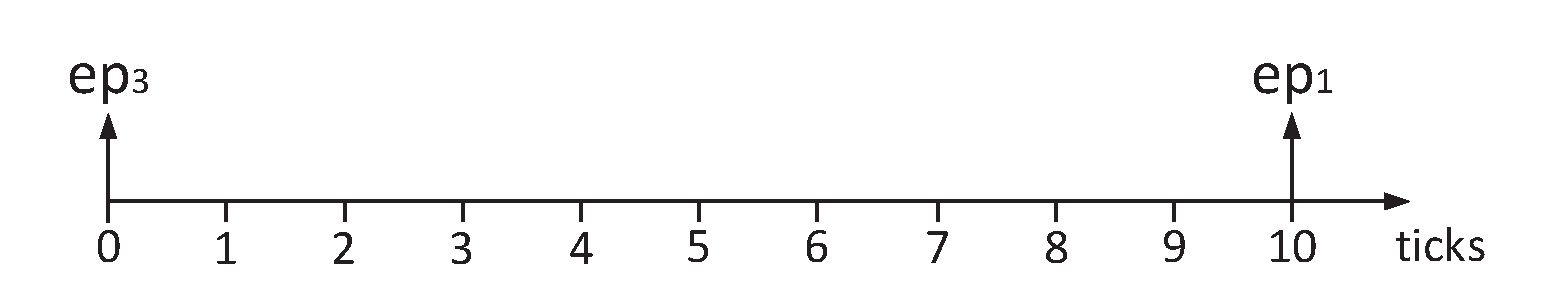
\includegraphics[scale=.34]{graphics/figure_combina1.eps}
    \caption{$ep_3$ expires at 0, $ep_1$ expires at 10. This time interval makes the computational requirement as $\omega_{l,r}^{(ep_3,0)}+\omega_{l,r}^{(ep_1,10)}$.}\label{figure_combination2}
  \end{subfigure}
  \caption{In a time interval with length 10, the computational requirement which is caused during scenario (b) is larger than it which is caused in scenario (a), i.e., the time interval in scenario (b) dominates it in scenario (a).}\label{figure_combination}
\end{figure}
As Figure \ref{figure_combination}, when $ep_3$ expires at the begin, this time interval always dominates others that make $ep_3$ the first appearance. Since a task could always keep time property if it keeps in the worst case, so we only need to consider the time interval which cannot be dominated. Regardless of the length of time interval, we can use $ep_3$ to denote this time interval, then represents the set of time interval which imply a series of offsets. So we replace offsets of a DST by its expiry points and replace $\delta(dst_1)\times\delta(dst_2)\times\dots\times\delta(dst_n)$ by combinations of expiry points.
\begin{definition}
For a set of DSTs $\tau=\{DST_1,DST_2,\dots,DST_n\}$, we use $\Phi$ to represent all combinations of expiry points of $\tau$.
\begin{equation}
  \Phi(\tau)=Node_1 \times Node_2\times\dots\times Node_n.
\end{equation}\label{equation_combination}
\end{definition}

%We pick one expiry point from each DST to form a set which is denoted by $\varepsilon\in\Phi$.
\subsection{Schedulability Analysis of Tasks}
As mentioned above, we analyze the schedulability by checking whether the time interval between activation and deadline of a task is big enough to accommodate the execution time of itself and other tasks which could interrupt it. But according to Section \ref{section_busywindow}, schedule situations before activation also make an impact. Therefore, we extend the time interval towards to before. This brings another question, "how far should we extend the time interval?" This answer has been given in Section \ref{section_busywindow}, i.e., the length we extended should not be more than the boundary of busy windows. Figure \ref{figure_3parts} shows the original time intervals with length $y$ and the extended time intervals with length $x+y$.
\begin{figure}
  \centering
  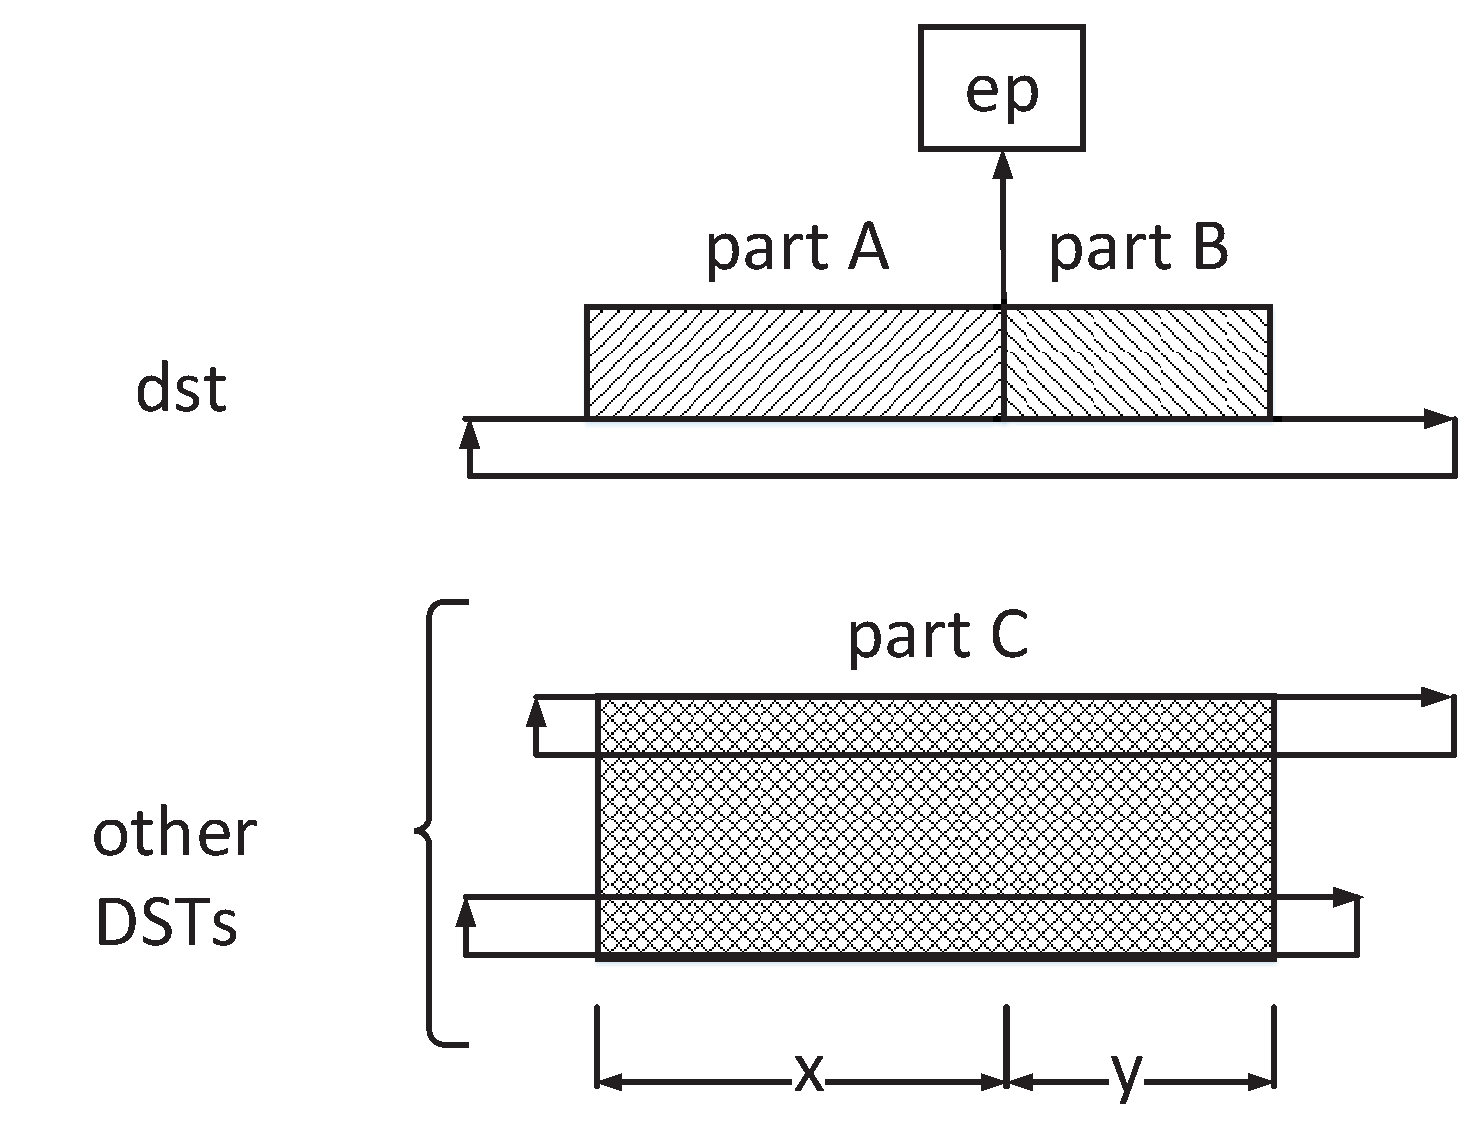
\includegraphics[scale=0.3]{graphics/figure_3parts.eps}
  \caption{An illustration of schedulability analysis of task $t$. There are three parts may affect the execution of $t$: A) interruption from $dst$ before task $t$ is activated, B) interruption from $dst$ after task $t$ is activated, C) interruption from other DSTs.}
  \label{figure_3parts}
\end{figure}

When several DSTs work concurrently, the influence on the execution of a task come from three parts: 1) tasks which are activated before this task from the same DST, 2) tasks which are activated after this task from the same DST, 3) tasks from other DSTs, cf. Figure \ref{figure_3parts}. The execution time of the three parts change base on $x$, $y$ and offsets between DSTs. After sorting out these three parts, we check whether the extended time interval could accommodate execution time of the task and interrupt time. Notice that we use prefix request function to calculate part B, but the expiry time of the first instance of expiry point in part B is $x$ instead of 0.


\begin{theorem}\label{theorem_testtask}
  For a finite set of DSTs $\tau$, if there is a $dst\in\tau$, expiry point $ep\in Node$, task $t\in Act(ep)$. Then task $t$ always meets its deadline if:
   \begin{equation}\begin{split}
      &\forall \varepsilon\in\Phi(\tau-\{dst\}),x\in[0,\sigma_l]:\exists y\in[e(lt),d(lt)]:\\
      srf^{ep}_{l(t)}(x)+&prf^{ep}_{l(t),-1}(y)-\omega_{l(t),-1}^{(ep,x)}
      +\sum\limits_{ep_i\in \varepsilon}prf^{ep_i}_{l(t),x}(x+y)\leq x+y.
    \end{split}\label{equation_verification}\end{equation}
\end{theorem}
\begin{proof}

  Firstly, we state that $\omega_{l(t),-1}^{(ep,x)}$ is the overlap between $srf^{ep}_{l(t)}$ and $prf^{ep}_{l(t),-1}$. Now, assuming Equation \ref{equation_verification} evaluates to false, but task $t$ always meets its deadline. Since Equation \ref{equation_verification} is false, there must exists a $\varepsilon\in\Phi(\tau-\{dst\})$ and a $x\leq \sigma_l$ makes the value of Equation \ref{equation_proof} is larger than $x+y$, where $y=0,1,2,\dots,d(t)$.
  \begin{equation}\begin{split}
      &\underbrace{srf^{ep}_{l(t)}(x)}_{part A}+\underbrace{prf^{ep}_{l(t),-1}(y)}_{part B}-\underbrace{\omega^{(ep,x)}_{l(t),-1}}_{overlap}+\underbrace{\sum\limits_{ep_i\in \varepsilon}prf^{ep_i}_{l(t),x}(x+y)}_{part C},
    \end{split}\label{equation_proof}\end{equation}
  
  Equation \ref{equation_proof} accumulates the execution time of task $t$ and all tasks could affect it, i.e., $t$ is the last task to be finished among them. Therefore, the minimal $y$ makes Equation \ref{equation_proof} not larger than $x+y$ is the worst-case responds time. But due to inexistence of $y\leq d(t)$ could satisfy Equation \ref{equation_verification}, so the WCRT exceed deadline. When expiry points in $\varepsilon$ expire $x$ ticks before the activation of $t$ contemporary, we find a situation that task $t$ could not meet its deadline, leading to a contradiction. 
  
  Now assuming Equation \ref{equation_verification} holds, but task $t$ may violates its deadline. If an instance of $t$ misses its deadline, there must exist a group of instances of tasks which could interrupt the execution of instance of $t$. We assume that the smallest activate time in this group is $x$ ticks smaller than activate time of the instance of $t$. According to Lemma \ref{lemma_busywindow}, $x\leq \sigma_l$. Since the Equation \ref{equation_verification} hold, the execution time caused by this group is less than or equal to $x+y$. So the task $t$ must be finished within $y$ ticks, which leading to a contradiction.
\end{proof}

%We illustrate this method as picking a task with lowest priority in this set of schedule tables, and verify whether this task could always meet its deadline, if the tasks pass verification, then pick another one. If all task pass verification, this set is declared as schedulable, if not, declared as non-schedulable.Verification of task is the foremost step in our method, so we give an overview of it: For a schedule table $st$ cotains expiry point $ep$, and $ep$ could activate task $t$, $t$ could always meets its deadline if other tasks always caues less than $d(t)-e(t)$ ticks interference in $d(t)$ ticks after releasing $t$.

\section{Schedulability analysis method}
In Section \ref{section_definition}, we have introduced some definition about schedulability analysis. In this section, we synthesize those definitions into an integrated method.

\subsection{Stages of Method}\label{section_8steps}
When a set of DSTs $\tau=\{dst_1,dst_2, \dots dst_n\}$ is given, the process of analyzing schedulability can be divided into stages as follows:
\begin{compactenum}
  %\item[1)]: Firstly, we calculate the hyperperiod of the set of DSTs .%Get hyperperiod

  \item: Picking one task with the lowest priority from $Task_1\cup Task_2\cup\dots\cup Task_n$ and denoting it as $lt$. %Find a task with the lowest priority
  \item: dividing $\tau$ into two parts: i) the one DST could activate $lt$, ii) the other DSTs. We denote them by $ldst$ and $other\_dsts$ respectively. %Divide the set of DSTs

  \item: Calculating the upper bound of busy windows for $l(lt)$ which is denoted by $\sigma_l$. The set of DSTs is non-schedulable if $\sigma_l$ exceed hyperperiod, .%Calculate boundary of busy window
  
  %Whenever determine one combination of start expiry point, need to set the release time of tasks those schedule table in $other\_st$ could activate, i.e., all tasks activate by start expiry point, set their release time to 0, release time of the rest of tasks are set according to the offset to start expiry point.
  \item: Picking one element $\varepsilon$ from $\Phi(other\_dsts)$, then we structure a path for every DSTs in $other\_dsts$: expire time of expiry points in $\varepsilon$ are setted as 0. The rest are structured according to delays of expiry points. We set the activate times of instances of tasks as well.%Set instances of tasks

  \item: Verifying whether the equation below could be satisfied, where $lep$ is the expiry point which could activate $lt$:%Verify schedulability in single combination
  \begin{equation}\begin{split}
      &\forall x\in[0,\sigma_l]:\exists y\in[e(lt),d(lt)]:\\
      srf^{lep}_{l(lt)}(x)+&prf^{lep}_{l(lt),-1}(y)-\omega^{(lep,x)}_{l(lt),-1}+\sum\limits_{ep_i\in\varepsilon}prf^{ep_i}_{l(lt),x}(x+y)\leq x+y
    \end{split}\label{equation_verify}\end{equation}
  
  \item: If Equation \ref{equation_verify} is satisfied, then we pick other $\varepsilon\in\Phi(other\_st)$ and repeat from step 4, until every elements in $\Phi(other\_st)$ have been picked, then we move to the next step. Instead, if there exist a situation makes Equation \ref{equation_verify} false, we declare this set of DSTs is non-schedulable.%Verify schedulability in all combination
  \item: Picking one task with the lowest priority in this set except tasks already passed verification. Then repeating the procedure from step 2.%Switch to another task
  \item: If all tasks pass validation, declaring this set is schedulable.%Declared schedulable
\end{compactenum}

\subsection{Integrated Method}
We summarize those steps and give two primary algorithms as below. We assume $\tau$ is a global variable which represents the set of DSTs, $task\_set$ is also a global variable which represents the set of all tasks in $\tau$.

\begin{algorithm}
  \caption{SCHEDULABILITY}
  \label{algorithm_schedulability}
  \begin{algorithmic}[1]
    \REQUIRE 
    \ENSURE schedulable or non-schedulable 
    \IF{$task\_set=\varnothing$}
    \STATE \Return schedulable
    \ELSE \STATE $lt \leftarrow GET\_LOWEST\_PRIORITY(task\_set)$\\$\qquad\qquad\qquad\backslash\backslash task\_set\ is\ a\ global\ variable$
    \IF{$pass=TASK\_SCHEDULABILITY\_ANALYSIS(lt)$}
    \STATE $task\_set\leftarrow task\_set-lt$
    \STATE \Return SCHEDULABILITY()
    \ELSE
    \STATE \Return non-schedulable 
    \ENDIF
    \ENDIF
  \end{algorithmic}
\end{algorithm}

At the begin of Algorithm \ref{algorithm_schedulability}, we implement line 1 and 2 to check whether the algorithm should terminate. Line 4 is corresponding to step 2 which aims to get the task with the lowest priority and divide $\tau$. We conceal the details of this function. The function $TASK\_VERIFY$ verifies whether a task always meets its deadline. If this function returns $pass$, then we will remove this task from $task\_set$ and continue run this algorithm. $task\_set$ is empty means all tasks have been confirmed to always meet its deadline. Therefore the set of DSTs is schedulable. Instead, if the return result of $TASK\_VERIFY$ is $not-pass$, that means $\tau$ is non-schedulable. The detail of $TASK\_VERIFY$ is shown in Algorithm \ref{algorithm_taskverify}.

\begin{algorithm}
  \caption{TASK\_SCHEDULABILITY\_ANALYSIS}
  \label{algorithm_taskverify}
  \begin{algorithmic}[1]
    \REQUIRE $lt$
    \ENSURE pass or not-pass
    \IF{$\sigma_l\leftarrow BOUNDARY(l(lt))>hyperperiod$}
    \STATE \Return not-pass
    \ELSE
    \FOR{$\forall\quad\varepsilon \in \Phi(other\_dsts)$}
    \FOR{$\forall\quad\ x\in[0,\sigma_l]$}
    \FOR{$\forall y\in[e(lt),d(lt)]$}
    \IF {$SRF^{lep}_{l(lt)}(x)+PRF^{lep}_{l(lt),-1}(y)-\omega^{(lep,x)}_{l(lt),-1}+$\\$\sum\limits_{ep_i\in\varepsilon}PRF^{ep_i}_{l(lt),x}(x+y)>x+y$}
    \STATE \Return not-pass
    \ENDIF
    \ENDFOR
    \ENDFOR
    \ENDFOR
    \STATE \Return pass
    \ENDIF
  \end{algorithmic}
\end{algorithm}

Algorithm \ref{algorithm_taskverify} aims to verify whether task $lt$ always meet its deadline. We use $lep$ to represent the expiry point which could activate $lt$. Firstly, we get the boundary of busy windows and compare with the hyperperiod. Line 4 to 7 is an implementment of Theorem \ref{theorem_testtask}. $SRF$ and $PRF$ represent the suffix request function and the prefix request function respectively. If the task $lt$ could not satisfy Equation \ref{equation_verification}, the algorithm returns $not-pass$, else returns $pass$.

\subsection{Demonstration}\label{section_demonstration}
As an example for this method, we construct a set of DSTs by uniting $dst_1$ in Figure \ref{figure_dst1}, $dst_2$ in Figure \ref{figure_dst2} and one more DST $dst_3$ in Figure \ref{figure_dst3}. In this case, the set of DSTs $\tau =\{dst_1,dst_2,dst_3\}$. Then we get the set of tasks, denote as $task\_set$: 
\[\begin{split}
task\_set=Tasks_1\cup Tasks_2\cup Tasks_3=\{t_1,t_2,t_3,t_4,t_5,t_6,t_7\}.
\end{split}\]

\begin{figure}
  \centering
  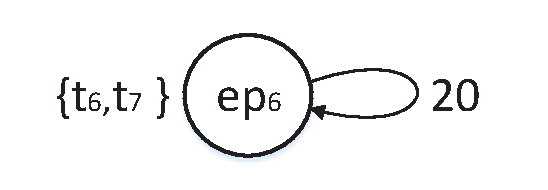
\includegraphics[scale=.4]{graphics/figure_dst3.eps}
  \caption{An example of DST $dst_3$, where $t_6=<2,11,6>,\ t_7=<1,3,4>$.} 
  \label{figure_dst3}
\end{figure}

Picking a task in $task\_set$ with the lowest priority, denoting as $lt$, assuming we choose $t_3$. Task $t_3$ divides $\tau$ into two parts: $dst_1$ and $\{dst_2,dst_3\}$, which are denoted by $ldst$ and $other\_dsts$ respectively. Then, we get the upper bound of busy windows for $l(t_3)$ by Equation \ref{equation_busywindow} and denote it as $\sigma_l$ = 13. The next step, we use $\Phi(\tau)$ to get all combinations of expiry points in $other\_dsts$ as $\{\{ep_4,ep_6\},\{ep_5,ep_6\}\}$. Assuming we pick $\varepsilon=\{ep_4,ep_6\}$ firstly. Then we build path $\rho_1=[(ep_4,0),(ep_5,3),(ep_4,14)\dots]$ for $dst_2$ and $\rho_2=[(ep_6,0),(ep_6,20),(ep_6,40),\dots]$ for $dst_3$. According to those paths, we set a series of instances of tasks like: $<1,3,3,0>$ and $<1,3,3,14>$ of $t_4$, $<2,11,6,20>$ of $t_6$, $<1,3,4,20>$ of $t_7$ and so on. Then we verify whether a $y\in(0,d(t_3)]$ exists for any $x\in[0,\sigma_l]$ to satisfy Equation \ref{equation_verify}, i.e.,
\[\begin{split}
&\forall x\in[0,13]:\exists y\in[2,9]:\\
srf^{ep_3}_6(x)+&prf^{ep_3}_{6,-1}(y)-\omega^{(ep_3,x)}_{6,-1}+\sum\limits_{ep_i\in \varepsilon}prf^{ep_i}_{6,x}(x+y)\leq x+y.
\end{split}\]


When x = 0, y = 9 satisfy the requirement, when x = 1, y =8 satisfy the requirement, ..., x = 13, y =3 satisfy the requirement. Then we verify other $\varepsilon$ until all elements in $\Phi(other\_dsts)$ pass validation and delete $t_3$ from $task\_set$. Then we continue pick another task with the lowest priority in $task\_set$ and repeat those steps. Finally, the algorithm will stop when $task\_set$ is empty or a situation could not pass verification.


\section{Experimental analysis}
In order to validate the effectiveness of our method, we setup an experiment to compare the result of our method and the execution on an implemented AUTOSAR OS. In this experiment, we develop a program to generate schedule tables randomly and implement them on the AUTOSAR while analyzing them by our algorithm. In this experiment, we use an industrial-used AUTOSAR operating system which is developed by iSoft Infrastructure Software Co., Ltd. Our target hardware platform is TC1782 32-Bit Single-Chip Microcontroller and more information about TC1782 in \cite{infineon.org}. 
\subsection{Experiment Setup}
We generate schedule tables subject to seven parameters as below. Table \ref{range} shows the ranges of parameters. 

\begin{compactitem}
  \item $st_{num}$, the number of schedule tables.
  \item $ep_{num}$, the maximal number of expiry points in a schedule table.
  \item $task_{num}$, the maximal number of tasks in an expiry point.
  \item $Delay$, the delay of an expiry point.
  \item $e(t)$, the execution time of a task.
  \item $d(t)$, the deadline of a task.
  \item $\delta$, the duration of schedule tables.
\end{compactitem}
\begin{table}[htbp]
  \centering
  \begin{tabular}{llllll}
    \toprule
    $st_{num}$ & $ep_{num}$ & $task_{num}$ & $Delay$ & $e(t)/d(t)$ & $d(t)/\delta$\\
    \midrule
    $[2,6]$&$[1,4]$&$[1,3]$&$[10,30]$&$[0,0.16]$&$[0.1,0.5]$\\
    \bottomrule
  \end{tabular}
  \caption{Ranges of parameters}\label{range}
\end{table}
%Except that, another goal of this generator is generating tasks randomly, we decide introduce slackness ratio $\eta$ to achieve that. We firstly define slackness on a task $t$ as $d(t)-e(t)$, 

After generating schedule tables randomly, we transform them into DSTs and consider them as the input of our method. Meanwhile we deploy those schedule tables into an implemented AUTOSAR by a configuration tool and test the schedulability. 

%This industrial-used AUTOSAR OS also provides a matched configuration tool to generate the configuration file and an user interface. We use this tool to generate configuration files follow up with our request and deploy our generated schedule tables into AUTOSAR by modifying the user interface. In order to implement deadline detection, we also setup an alarm for each task, which will expire when task's on deadline. The alarm is assigned to a callback routine which could check the state of the corresponding task. If the state is not suspended, i.e., this task is not finished yet, the callback routine will return false. If the state is suspended, the callback routine will return true. With those alarms, we could find the task which violates deadline as soon as time faults raises. 

\subsection{Consistency Analysis} 
%We introduce a new feature utilization $\eta$ to assist our comparison. For a schedule table $st$ 
%\[\eta=\frac{\sum\limits_{ep_i\in Node(st)}\sum\limits_{t_i\in Act(ep_i)}e(t_i)}{\delta}\] 
%i.e., ratio of sum of all tasks' execution time in st to duraiton of st.
The experiment of comparison shows that the result of our method all compared exactly to an actual running situation on the implemented AUTOSAR. Several examples and their result are synthesized in Table \ref{table_compare}. We use $task_{sum}$ to represent the amount of tasks. %($\sum\eta$ represent the sum of utilization of all schedule tables, it's obviously not schedulable when this value exceed 100).


\begin{table}[htbp]
  \centering
  \begin{tabular}{llllll}
    \toprule
    &&\multicolumn{2}{c}{Schedulability}\\
    \cmidrule{3-4}
    $st_{num}$ & $task_{sum}$ & our method & industrial OS\\
    \midrule
    3&14&Invalid&Invalid\\
    4&28&  Valid&    Valid\\
    5&36&Invalid&Invalid\\
    6&27&Invalid&Invalid\\
    %9&33&TIME OUT&NOT valid\\10&100&TIME OUT&NOT valid\\
    
    \bottomrule
  \end{tabular}
  \caption{Comparison of schedulability analysis result}
  \label{table_compare}
\end{table}

If the schedulability result obtained by our method is non-schedulable, an amending advice will be given. For example, when we test task $t_7$, Equation \ref{equation_verification} could not be satisfied when $x=0$ and $\varepsilon={ep_4,ep_6}$. Then we try to widen it's deadline from 3 ticks to 4 and test $t_7$ again. Until it pass validation. 
%cf. Figure \ref{figure_widen}. 
Then we modify any tasks could not pass validation. Finally, we get an amended example, which is schedulable and it is schedulable on implemented AUTOSAR as well.

%\begin{figure}
%  \centering
%  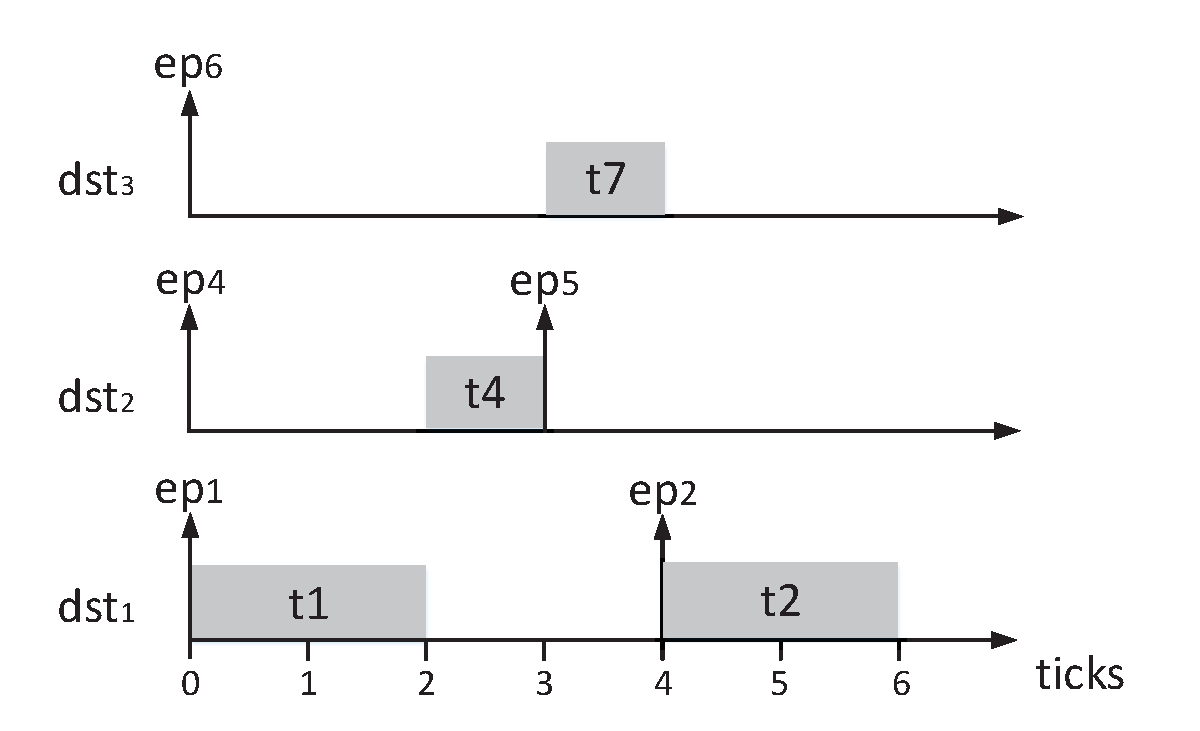
\includegraphics[scale=.45]{graphics/figure_widen.eps}
%  \caption{$t_7$ is activated by $ep_6$ at 0. But $t_7$ could not be finished until 4, which makes $t_7$ violates it's deadline.}
%  \label{figure_widen}
%\end{figure}

\section{Conclusion}
In this paper, we have abstracted the behaviors of schedule tables as formal models and proposed an algorithm based on the models. Our algorithm is to analyze the schedulability of AUTOSAR OS by travelling all the possible offsets between schedule tables. Moreover, we conduct an experiment, which runs a set of testbench on an industrial AUTOSAR OS and the experiment respectively to check the effectiveness of our method. Through the comparison result, we believe that our method could perform well in assisting developers in designing schedule tables.
 
This work has gotten a promising result in analyzing AUTOSAR OS on uniprocessor. Since AUTOSAR specification has introduced multicore operating systems, we are considering to work on schedulability analysis of them. Besides, schedulability analysis for extended tasks, which are allowed to synchronize through setting and waiting events, is another interesting topic we would like to pursue.


%\bibliographystyle{ACM-Reference-Format}
\bibliographystyle{unsrt}
\bibliography{myreference}

\end{document}
